\documentclass[a4paper,12pt]{report}

\usepackage[T2A]{fontenc}
\usepackage[english,russian]{babel}
\usepackage[utf8]{inputenc}
\usepackage[titletoc]{appendix}
\usepackage[usenames, dvipsnames]{xcolor}
\usepackage{float}
\usepackage{listings}
\usepackage[ruled,vlined]{algorithm2e}
%\usepackage{pscyr}
\usepackage{graphicx}
%\usepackage{amstext}
%\usepackage{amssymb}
% \usepackage{lscape}
% \usepackage{xcolor}
\usepackage{verbatim}
\usepackage{caption}
\usepackage{adjustbox}

\usepackage{etoolbox}

\usepackage{mathtools}
\DeclarePairedDelimiter{\ceil}{\lceil}{\rceil}
\DeclarePairedDelimiter\floor{\lfloor}{\rfloor}

\usepackage{numprint}
\usepackage{totcount}
\usepackage{xassoccnt}


\newcounter{truechapters}
\regtotcounter{truechapters}

\newcounter{totalchapters}
\newcounter{appendixchapters}
\DeclareAssociatedCounters{chapter}{totalchapters,appendixchapters}
\regtotcounter{totalchapters}
\regtotcounter{appendixchapters}

\preto\appendix{%
  % save the number of true chapters
  \setcounter{truechapters}{\value{chapter}}%
  % reset the number of chapters
  \setcounter{appendixchapters}{0}%
}

\newtotcounter{figurecnt}
\def\oldfig{} \let\oldfig=\figure
\def\figure{\stepcounter{figurecnt}\oldfig}
%таблиц (only longtable)
\newtotcounter{tablecnt}
\def\oldtab{} \let\oldtab=\longtable
\def\longtable{\stepcounter{tablecnt}\oldtab}
% \def\table{\stepcounter{tablecnt}\oldtab}

\newtotcounter[auxfile=totals.aux]{bibcnt}
\def\oldbibitem{} \let\oldbibitem=\bibitem
\def\bibitem{\stepcounter{bibcnt}\oldbibitem}
\regtotcounter[auxfile=totals.aux]{page}

% \newcommand{\No}{\textnumero}


% \PassOptionsToPackage{unicode=true}{hyperref} % options for packages loaded elsewhere
% \PassOptionsToPackage{hyphens}{url}
% % use upquote if available, for straight quotes in verbatim environments
% \IfFileExists{upquote.sty}{\usepackage{upquote}}{}
% % use microtype if available
% \IfFileExists{microtype.sty}{%
% \usepackage[]{microtype}
% \UseMicrotypeSet[protrusion]{basicmath} % disable protrusion for tt fonts
% }{}
% \IfFileExists{parskip.sty}{%
% \usepackage{parskip}
% }{% else
% \setlength{\parindent}{0pt}
% \setlength{\parskip}{6pt plus 2pt minus 1pt}
% }


% PDF search & cut'n'paste
\usepackage{cmap}
\usepackage{url}
\usepackage{textcomp}
\usepackage[colorlinks]{hyperref}
\hypersetup{
            pdfborder={0 0 0},
            breaklinks=true}
\urlstyle{same}  % don't use monospace font for urls
\usepackage{longtable,booktabs}

\lstset{
	language=C,
	tabsize=4,
	breaklines=true,
	basicstyle=\footnotesize,
	identifierstyle=\ttfamily,
	extendedchars=true,
}


\lstnewenvironment{C_LANG}[1][]{
    \lstset{
      belowcaptionskip=1\baselineskip,
      breaklines=true,
      frame=L,
      xleftmargin=\parindent,
      language=C,
      showstringspaces=false,
      basicstyle=\footnotesize\ttfamily,
      keywordstyle=\bfseries\color{green!40!black},
      commentstyle=\itshape\color{purple!40!black},
      identifierstyle=\color{blue},
      stringstyle=\color{orange},
    \lstdefinestyle{nonumbers}
    {numbers=none}
}{}


\lstnewenvironment{cpp_code}[1][]{
    \lstset{
        language=C++,
        numbers=left,
        stepnumber=1,
        breaklines=true,
        basicstyle=\linespread{1.0}\ttfamily,
        keywordstyle=\color{blue}\ttfamily,
        stringstyle=\color{red}\ttfamily,
        commentstyle=\color{OliveGreen}\ttfamily,
        morecomment=[l][\color{magenta}]{\#}
        columns=fullflexible,
        postbreak=\mbox{\textcolor{red}{$\hookrightarrow$}\space},
        escapeinside={(*@}{@*)},
        showstringspaces=false
    }
    \lstdefinestyle{nonumbers}
    {numbers=none}
}{}

    
\lstnewenvironment{py_code}[1][]{
    \lstset{
        language=python,
        stepnumber=1,
        breaklines=true,
        basicstyle=\linespread{1.0}\ttfamily,
        keywordstyle=\color{blue}\ttfamily,
        stringstyle=\color{red}\ttfamily,
        commentstyle=\color{OliveGreen}\ttfamily,
        morecomment=[l][\color{magenta}]{\#}
        columns=fullflexible,
        otherkeywords={self},
        postbreak=\mbox{\textcolor{red}{$\hookrightarrow$}\space},
        escapeinside={(*@}{@*)},
        showstringspaces=false,
    }
    \lstdefinestyle{nonumbers}
    {numbers=none}
}{}

\lstnewenvironment{code}[1][]{
    \lstset{
        language=bash,
        breaklines=true,
        basicstyle=\linespread{1.0}\ttfamily,
        keywordstyle=\color{blue}\ttfamily,
        stringstyle=\color{red}\ttfamily,
        commentstyle=\color{OliveGreen}\ttfamily,
        morecomment=[l][\color{magenta}]{\#}
        columns=fullflexible,
        postbreak=\mbox{\textcolor{red}{$\hookrightarrow$}\space},
        escapeinside={(*@}{@*)},
    }
    \lstdefinestyle{nonumbers}
    {numbers=none}
}{}

\lstset{
    language=python,
    breaklines=true,
    basicstyle=\linespread{1.0}\ttfamily,
    keywordstyle=\color{blue}\ttfamily,
    stringstyle=\color{red}\ttfamily,
    commentstyle=\color{OliveGreen}\ttfamily,
    morecomment=[l][\color{magenta}]{\#}
    columns=fullflexible,
    postbreak=\mbox{\textcolor{red}{$\hookrightarrow$}\space},
    escapeinside={(*@}{@*)},
}

\makeatletter
\renewcommand\paragraph{\@startsection{paragraph}{4}{\z@}%
            {-2.5ex\@plus -1ex \@minus -.25ex}%
            {1.25ex \@plus .25ex}%
            {\normalfont\normalsize\bfseries}}
\makeatother

\setcounter{secnumdepth}{3} % how many sectioning levels to assign numbers to
\setcounter{tocdepth}{4}    % how many sectioning levels to show in ToC
\renewcommand{\rmdefault}{ftm}
% \renewcommand{Оглавление}
\linespread{1.3} %1.5 межстрочный интервал
\usepackage[left=3cm,right=2.5cm,top=3cm,bottom=3cm,bindingoffset=0cm]{geometry}



\begin{document}


\begin{titlepage}
	\begin{center}
	\textsc{\normalsize{ФЕДЕРАЛЬНОЕ ГОСУДАРСТВЕННОЕ АВТОНОМНОЕ ОБРАЗОВАТЕЛЬНОЕ}}\\
\textsc{\normalsize{УЧРЕЖДЕНИЕ ВЫСШЕГО ОБРАЗОВАНИЯ}}\\
\textsc{\normalsize{НАЦИОНАЛЬНЫЙ ИССЛЕДОВАТЕЛЬСКИЙ УНИВЕРСИТЕТ}}\\
\textsc{\normalsize{{«ВЫСШАЯ ШКОЛА ЭКОНОМИКИ»}}\\
	\normalsize{ФАКУЛЬТЕТ КОМПЬЮТЕРНЫХ НАУК}}
	\\[.5cm]
	\normalsize{\underline{Дьячков Леонид Андреевич}}\\[.5cm]

	\normalsize{МАГИСТЕРСКАЯ ДИССЕРТАЦИЯ}\\[.8cm]

	{\normalsize {\ul{\textbf{Исследование и разработка методов динамического анализа для определения входных данных влияющих на выполнение условных переходов}}}} \\[.3cm]
	{\normalsize {\ul{\textbf{Research and Development of Methods of Dynamic Analysis for Detecting Input Data Affecting Condition Branches Execution}}}}\\[.5cm]

	по направлению подготовки \underline{09.04.04 Программная инженерия}\\
	образовательная программа \underline{«Системное программирование»}

	\begin{flushleft}
	Cтудент\\
	\underline{\hspace{3cm}}\\
	Л.А. Дьячков\\
	\end{flushleft}
	\begin{flushright}
		
		Научный руководитель: \\ 
		д.ф.-м.н, проф. \\
		\underline{\hspace{3cm}}\\
		А.К. Петренко \\
		\\
		Соруководитель: \\ 
		к.ф.-м.н, с.н.с ИСП РАН \\
		\underline{\hspace{3cm}}\\
		Ш.Ф. Kурмангалеев \\
	\end{flushright}
	\vfill
	
	Москва, 2019
	\end{center}

\end{titlepage}

\frontmatter
% \begin{eabstract}
% ...
% \end{eabstract}

\begin{abstract}
В настоящее время фаззинг-тестирование -- активно развивающийся метод для поиска ошибок в программном обеспечении \cite{DBLP:journals/corr/abs-1808-09700}. Тем не менее, у него имеется ряд недостатков, в частности достижение некоторых фрагментов кода может быть затруднено. Для решения этой проблемы фаззеру необходимо знать какие входные данные влияют на выполнение условных переходов. Получить необходимую информацию можно при помощи динамического анализа. В данной работе приводится обзор подходов, позволяющих решать эту задачу, а также подходящих инструментов динамического анализа. Кроме того, были предложены и разработаны методы на основе динамического анализа помеченных данных и динамического символьного выполнения. 

Работа содержит \total{page} страницу, \total{truechapters} \total{totalchapters} главы, \total{figurecnt} рисунков, \total{tablecnt} таблицу, \total{bibcnt} источников, \total{appendixchapters} приложения.
\end{abstract}

\tableofcontents
\chapter{Введение}


В последние годны наблюдается заметный рост количества уязвимостей в программном обеспечении. Так, согласно статистике \cite{CVEstats}, в $2016$ году было обнаружено $6447$ уязвимостей, в $2017$ --  $14714$, a в $2018$ -- $16555$. Это связано как с объемом и сложностью, разрабатываемого программного обеспечения, так и с развитием техник тестирования безопасности.

\begin{figure}[h]
    \center{
        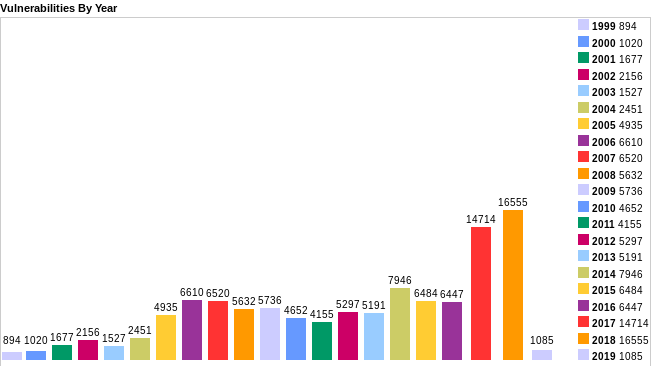
\includegraphics[scale=0.5]{img/cve_stats.png}
    }
    \caption{Cтатистика опубликованных уязвимостей за последние 20 лет}
    \label{fig:image}
\end{figure}

Одним из популярных подходов к автоматизации поиска уязвимостей является фаззинг-тестирование. Это
техника тестирования программного обеспечения, заключающая в передаче приложению на вход неправильных, неожиданных или случайных данных.

P

Фаззинг-тестирование является достаточно популярным подходом в тестировании на безопасность.


В последние годы наблюдается рост интереса к фаззинг-тестированию.



\chapter{Обзор}

% \chapter{Методы реализации динамического анализа}

\section{Динамический Анализ}

Динамический анализ - это анализ, заключающийся в непосредственном выполнении кода. Однако, просто запустить программу может быть недостаточно. Существует несколько способов получения дополнительной информации во время выполнения:

\begin{itemize}
\item {\em Исполнение кода в виртуальном окружении}. При данном подходе программа запускается внутри некоторого программного эмулятора. Например qemu \cite{QEMU}.
%\item $\sigma$ is a {\em symbolic store} that associates program variables with expressions over \mynote{[D] $\alpha_i$ also concrete?} concrete and symbolic values $\alpha_i$.

\item {\em Статическая инструментация}.
Статическая инструментация бывает двух видов.
    \begin{itemize}
        \item {\em Статическая инструментация исходного кода}. В случае, если имеется доступ к исходному коду, можно просто внести изменения в текстовые файлы с кодом. Добавление отладочной печати может быть примером статической инструментации исходного кода. Подобный вид инструментации также поддерживается непосредственно компилятором. Так GCC имеет опцию  \textit{-finstrument-functions}
        \item {\em Статическая инструментация бинарного кода (SBI)}. В случае отсутствия исходного кода, изменениям может быть подвержен сам исполняемый файл на диске. Тривиальным примером такой инструментации может быть например замена условных переходов на \textint{nop} инструкции. 
    \end{itemize}

\item {\em Динамическая инструментация}. Данный вид инструментации позволяет вносить изменения в программу непосредственно в процессе её выполнения. Этот метод будет рассмотрен далее подробнее, как наиболее популярный среди инструментов, использованных в данной работе.


\section{Динамическая бинарная инструментация}

Рассмотрим несколько популярных DBI инструментов.

\subsection{Valgrind}
...

\subsection{Pin}
...

\section{Анализ помеченных данных}

Динамический анализ помеченных данных (Dynamic Taint Analysis, DTA), также известный как динамический анализ потока данных (Dynamic Flow tracking, DFT)(DFT) - это техника анализа програм, позволяющая определить какие состояния программы зависят от входных данных.
% Существует также статический анализ потока данных

Примером классической задачи, решаемой при помощи анализа помеченных данных, может служить задача определения достигают ли данные из недоверенного источника "Опасных" функций. Многие уязвимости в программном обеспечении обусловлены недостаточным контролем над входными данным. Применение анализа потока данных позволяет детектировать подобные проблемы.

Динамический анализ помеченных данных делится на 3 фазы

    \begin{itemize}
        \item {\em Определение источников помеченных данных}. На данном этапе определяется каким данные должны быть помечены. Обычно метками снабжаются данные, получаемые из недоверенного
        источника. В зависимости от типа приложения, это могут быть данные полученные по сети, из файла, или потока стандартного ввода.
        \item {\em Распространение пометок (Taint propogation)}. Для отслеживания потока данных, 
        для каждой инструкции манипулирующей данными необходимо написать инструментирующий код для манипуляции метками. Так, например инструкция \textint{mov eax, ebx} перезаписывает метку для регистра eax меткой регистра \textint{ebx}. Это фаза является самой сложной, поскольку оставляет много открытых вопросов. К примеру
        \begin{itemize}
            \item Следует ли отслеживать помеченность побайтово или побитого? Если \textint{eax} помечен, то после команды \textint{or eax, 0x746567bc} контролируются уже не все биты. Однако, в большинстве случаев отслеживание каждого бита может быть слишком дорогой операцией.
            \item Следует ли помечать адрес памяти, на который указывает помеченная переменная?
            \item Если условный переход зависит от помеченных данных, следует ли считать что последующие инструкции тоже от них зависят?
            \item Как хранить информацию о помеченных адресах в памяти?
            \item Cледует ли различать пометки, полученные из разных источников?
        \end{itemize}
        \item {\em Применение политик безопасности}. Фаза, на которой используются результаты анализа. Происходящее на этом этапе зависит от изначальных целей анализа. Типичным примером может быть отслеживание попадания помеченных данных в аргументы некоторых заранее выделенных функций, или факта помеченности счетчика инструкций.
    \end{itemize}


% \section{методы реализации технологии анализа помеченных данных}
Рассмотрим несколько подходов к реализации анализа помеченных данных.

% \subsection{Символьное выполнение}

\subsection{Множество помеченных адресов}

\subsection{Хэш таблица с побайтовыми метками}

\section{Символьное выполнение}


\section{Обзор технологий динамического анализа}

\section{Triton}

\section{angr}

\section{manticore}

\section{taintgrind}

\section{libdft}

\section{moflow}



\chapter{Сравнение инструментов для динамического анализа}

\section{Библиотека для снятия и анализа трас}

\section{Результаты сравнение}

\section{Выводы}




\chapter{Методы определения входных данных влияющих на условные переходы}

% Для начала расмотрим самый простой способ

\section{Использование символьного выполнение}

% Символьное выполнение


\section{Использование меток помеченных данных}

\section{Комбинированный подход}

Оба предыдыщих подхода имеют недостатки. Построение символьных формул для всех инструкций может быть достаточно ресурсоемкой задачей. Время работы \em{Triton} может быть тому примером. В случае же, если используется онлайн символьное выполнение - проблема стоит еще острее, так \em{angr} вообще оказывается не очень применим на программах размером больше чем задания для CTF соревнований.
\\
С другой стороны, многие технологии анализа помеченных данных не поддерживают гранулярность на уровне отдельных байт, и возможность отследить от каких именно входных байт зависит некоторый адрес или регистр отсутствует. Даже если есть возможность отследить метки на каждый байт, существуют примеры когда этого недостаточно. так в \cite{Cavallaro07anti-taint-analysis:practical} приводится следующий пример, где между x и y есть взаимно-однозначное соответствие, которое не отслеживается динамическим анализом помеченных данных.
\\

\begin{lstlisting}[environoment=C_LANG]
char y[256], x[256];
...
int n = read(network, y, sizeof(y));
for (int i=0; i < n; i++) {
    switch (y[i]) {
        case 0: x[i] = (char)13; break;
        case 1: x[i] = (char)14; break;
        ...
        case 255: x[i] = (char)12; break;
        default: break;
    }
}
\end{lstlisting}

\chapter{Прототипы решающие задачу}

\section{Решение на основе Angr}

\section{Решение на основе Moflow}

\chapter{Заключение}
% \subsection 




 % Для решения этой проблемы может использоваться динамическое символьное выполнение, например Driller для фаззера afl \cite{DRILLER}. Для улучшения работы фаззера
\mainmatter
\chapter{Методы определения входных данных влияющих на условные переходы}

% В данной главе предлагаются два метода, основанный на символьном вы

% Для решение поставленной задачи необходимо:

% \begin{itemize}
%     \item Для каждого байта
%     \item 
% \end{itemize}

% https://www.usenix.org/system/files/conference/usenixsecurity13/sec13-paper_haller.pdf

% https://minemu.org/

% https://sites.cs.ucsb.edu/~vigna/publications/2016_SP_angrSoK.pdf

% https://www.cs.vu.nl/~herbertb/papers/borg_codaspy15.pdf

% Для начала расмотрим самый простой способ

\section{Использование символьного выполнения}

Первое что необходимо сделать, это установить соответствие между символьными переменными и байтами входного файла. Эта задача может быть решена двумя разными способами, в зависимости от используемых технологий.

\begin{itemize}
    \item В случае если используемый фреймворк предоставляет абстракцию вида ``Символьный файл'', можно просто ей воспользоваться. Символьный файл уже содержит в себе символьный массив байт, соответствующий байтам исходного файла.
    \item В противном случае необходимо использовать механизм перехвата системных вызовов. Для начала следует отслеживать вызовы \texttt{open} и \texttt{openat}, в случае если их аргумент соответствует имени отслеживаемого файла полученный дескриптор и его текущее смещение заносится в множество отслеживаемых дескрипторов. При вызове \texttt{lseek} для соответствующего дескриптора изменяется смещение, а при вызове \texttt{close} -- дескриптор удаляется из множества. Для вызовов \texttt{read} и \texttt{pread64} создаются символьные переменные, в хэш-таблицу помещается информация о соответствии байт файла. Аналогичным образом обрабатывается и работа с \texttt{mmap}.
\end{itemize}


Метод на основе динамического символьного выполнения основывается на использовании предиката пути.
Его конструирование основывается на трансляции инструкций ассемблера или промежуточного языка в формулы для SMT решателя, и выполняется существующими инструментами автоматически.
При обработке инструкции условного перехода извлекается формула соответствующая конъюнкции формул для соответствующих флагов, определяющих условный переход, после чего производится её конъюнкция с существующим предикатом пути.

Важно отметить, что предикат пути представим в виде абстрактно-синтаксического дерева. Это обусловлено тем, что уравнения для SMT-решателей в формате SMT-Lib2 представляют собой S-выражения. При этом в листьях дерева могут находиться или константы, или символьные переменные. Отсюда вытекает следующий алгоритм.
\bigskip

\begin{algorithm}[H]
\SetAlgoLined
\KwIn{Предикат пути, представленный в виде AST для SMT формулы}
\KwOut{Список символьных переменных}
\SetKwFunction{getleafs}{\textbf{GetLeafs}}
\SetKwFunction{issymvar}{\textbf{IsSymVar}}
\SetKwFunction{isconstant}{\textbf{IsConstant}}
\SetKw{continue}{\textbf{continue}}
% \Indm\nonl\printlcs{$V$}\\
% \KwResult{Write here the result
\SetKwProg{Fn}{Function}{:}{}
\Fn{\getleafs{$V$}}{
$Found \gets \emptyset$\;
  \For{$child \in V$} {
    \If{$\issymvar ( child ) $} {
        $Found \gets Found \cup \{ child \}$\;
    } \ElseIf{$\isconstant ( child ) $} {
        $\continue$\;
    }
    \Else {
      $Found \gets Found \cup \getleafs{child}$\;
    }
  }
  \Return{$Found$}\;
}
  \caption{Метод на основе символьного выполнения}
\end{algorithm}

\bigskip
Поскольку соответствие символьных переменных смещениям в файле известно~--- задача решена.

Однако существует еще одна проблема~--- предикат пути содержит условие на весь путь до данной точки, в то время как для решаемой задачи интерес представляет только его часть, отвечающая за последний переход.


Для решения этой проблемы вместо того, чтобы использовать сам предикат пути можно отслеживать события, заключающиеся в добавление в него новых условий и работать уже непосредственно с ними (добавление происходит в момент когда встречается условный переход). В случае \texttt{Angr} подобное решение достаточно легко реализуемо.

Данное решение обладает следующими преимуществами:
  \begin{itemize}
    \item Простой и понятный алгоритм
    \item Высокая точность работы (возможно достижение побитовой точности)
  \end{itemize}

При этом наличествуют следующие недостатки:
\begin{itemize}
  \item Низкая производительность (Построение формул на каждую инструкцию)
  \item Ни один из рассмотренных инструментов инструментов не позволяет реализовать метод, работающий на несинтетических примерах без ощутимых доработок самого инструмента.
\end{itemize}

Относительно пункта про производительность можно сделать несколько замечаний.
Во-первых, существует оптимизация, доступная например в \texttt{Triton}. Для того, чтобы сократить количество генерируемых уравнений можно использовать слайсинг по помеченным данным.
Во-вторых, с учетом замедления вносимого построением формул на каждую инструкцию, может быть целесообразнее непосредственно решать предикат пути и генерировать соответствующие входные данные.

\subsection{Решение на основе Angr}

Наиболее быстро вышеописанный метод можно реализовать на основе \texttt{Angr}. Несмотря на то, что само по себе полученное решение не применимо для крупных программ, полученный прототип хорошо иллюстрирует работу метода и его практическую применимость.

Полный программный код предложенного решения можно найти в приложении \ref{angrimpl}, ниже приводится пример его работы на простом примере.

\begin{lstlisting}[environoment=C_LANG, caption=jumper.c, label={lst:jumper}, captionpos=b]
int main(int argc, char** argv)
{
    char buff[SIZE];
    FILE *file1, *file2;
    file1 = fopen("input1", "r");
    file2 = fopen("input2", "r");
    fseek(file1, 10, SEEK_SET);
    if (!fread(buff, sizeof(char), 7, file1)) {
        return error_handler();
    }
    if (!fread(buff, sizeof(char), 2, file2)) {
        return error_handler();
    }
    if (buff[0] == 'a') {
        if (buff[3] == 'b') {
            loc1();
        } else if (buff[5] < buff[6]) {
            loc2();
        } else if (buff[2] >= buff[1]) {
            loc3();
        }
        loc4();
    }
    loc5();
    puts(buff);
}
\end{lstlisting}


Поскольку \texttt{Angr} использует онлайн поиск и поддерживает символьные файлы в качестве входного аргумента используется только имена файлов и адрес, путь к которому следует найти.

\begin{lstlisting}[caption=Интерфейс инструмента основанного на angr, captionpos=b]]
usage: taint_influence.py [-h] [-s] [-S FILE_SIZE] [-f FILES [FILES ...]]
                  binary func [args [args ...]]

Get tainted bytes for branches

positional arguments:
  binary                binary to analyse
  func                  function or adress to search
  args                  argv for program to analyse

optional arguments:
  -h, --help            show this help message and exit
  -s, --symbolic_argv   symbolize argv if set
  -S FILE_SIZE, --file-size FILE_SIZE
                        Size of symbolic files
  -f FILES [FILES ...], --files FILES [FILES ...]
                        list of files to symbolize
\end{lstlisting}

Ниже приводится пример работы инструмента, запущенного следующей строкой \texttt{taint\_influence.py jumper loc3 file -f input1 input2 -S 20}

\begin{lstlisting}[caption=Пример работы инструмента,captionpos=b]
=====Trace=========
------------------------------
Basic block addr: 0x401300
Instruction addr: 0x40130a
Formula: <Bool ((input1_40_160[63:56] - input2_41_160[151:144])[7:7] ^ ((input1_40_160[63:63] ^ input2_41_160[151:151]) & (input1_40_160[63:63] ^ (input1_40_160[63:56] - input2_41_160[151:144])[7:7]))) == 0>
Tainted bytes: {'input2': {1}, 'input1': {12}}


------------------------------
Basic block addr: 0x4012e8
Instruction addr: 0x4012f2
Formula: <Bool ((input1_40_160[39:32] - input1_40_160[31:24])[7:7] ^ ((input1_40_160[39:39] ^ input1_40_160[31:31]) & (input1_40_160[39:39] ^ (input1_40_160[39:32] - input1_40_160[31:24])[7:7]))) == 0>
Tainted bytes: {'input1': {16, 15}}


------------------------------
Basic block addr: 0x4012d4
Instruction addr: 0x4012da
Formula: <Bool input1_40_160[55:48] != 98>
Tainted bytes: {'input1': {13}}


------------------------------
Basic block addr: 0x4012cc
Instruction addr: 0x4012d2
Formula: <Bool input2_41_160[159:152] == 97>
Tainted bytes: {'input2': {0}}


===files====
<BV160 input1_40_160>
b'\x00\x00\x00\x00\x00\x00\x00\x00\x00\x00\x00\x00\x00\x9d\x00\x00\x00\x00\x00\x00'
<BV160 input2_41_160>
b'a\x00\x00\x00\x00\x00\x00\x00\x00\x00\x00\x00\x00\x00\x00\x00\x00\x00\x00\x00'
\end{lstlisting}

Как можно видеть, инструмент корректно выводит байты влияющие на выполнение условного перехода. Кроме того \texttt{Angr} позволяет сгенерировать конкретные файлы на которых программа достигает интересующей инструкции.

% предикат пути представляется в виде конъюнкции предикатов
% поскольку одной из основных задач соответсвтующих инструментов является его конструирование

% каждому байту входного файла ставится в соответствие символьная переменная.
% для каждого предиката пути выполняется следующий алгоритм


% поскольку переменные взаимнооднозначно соответствуют адресам -- задача решена.

% \subsection{решение на основе angr}


\section{Использование анализа помеченных данных}
\label{taintmethod}

Метод на основе анализа помеченных данных во многом похож на метод с динамическим символьным выполнением. Так, первое что необходимо сделать -- корректно реализовать помечивание источников входных данных. Абстракций вроде символьного файла в случае анализа помеченных данных нет, поэтому используется механизм перехвата системных вызовов.

Первым делом встает вопрос о гранулярности меток. Использования гранулярности меньше байта не целесообразно, поскольку заметно влияет на производительность, в то время как точность в любом случае теряется. Например рассмотрим инструкцию \texttt{pcmpeqb xmm2, xmm1}, после выполнения этой инструкции \texttt{xmm2} должен содержать метки, относящиеся к обоим регистрам. Учесть какие именно биты повлияли на результат можно только методами символьного выполнения.
Использование побайтовых меток является приемлемым решением, тем не менее может иметь смысл использовать информацию о структуре файла, если она заранее известна для разметки. Так, при помощи утилиты \texttt{afl-analyze} можно узнать байты, отвечающие за некоторую контрольную сумму. Разумно пометить её одним тегом. В \cite{Angora} также предлагается использовать информацию о типах переменных, и проводить размечивание с учетом их размера. Данный подход требует предварительного статического анализа исходного кода или бинарного кода.

Кроме того, необходимо поддерживать неограниченное количество различных пометок для участка памяти. Это достаточно очевидное требование для поставленной задачи, но оно совсем не актуально для классической задачи анализа помеченных данных\footnote{Попадают ли данные из недоверенных источников в ``опасные'' функции}, поэтому оно не выполняется в большинстве рассмотренных в данной работе инструментов.

В алгоритме распространения пометок следует помечать данные лежащие по помеченным адресам, при этом не следует производить распространение пометок по управлению, подобный подход позволяет сохранить разумный баланс между ложнопомеченными и недопомеченными данными.

Само определение данных влияющих на условный переход сводится к тому, чтобы определить метки соответствующие регистру флагов непосредственно перед обработкой инструкции условного перехода.

Если резюмировать, алгоритм на основе анализа помеченных данных выглядит так:

\begin{itemize}
  \item Каждому байту входного файла ставится в соответсвие метка (тег).
  \item Для всех последующих инструкций в трассе выполнение выполняется алгоритм распространения пометок
  \item Для каждой инструкции условного перехода извлекаются теги, которыми помечен регистр флагов. Байты, соответствующие этим тегам -- искомые.
\end{itemize}

К достоинствам описанного метода можно отнести его достаточно простую реализацию\footnote{В предположении, что уже имеется достаточно хороший инструмент для анализа помеченных данных} и высокую, по сравнению с символьным выполнением, скорость.

К недостаткам можно отнести худшую по сравнению с символьным выполнением точность. Например в \cite{Cavallaro07anti-taint-analysis:practical} приводится следующий пример.

\begin{lstlisting}[environoment=C_LANG,captionpos=b]
char y[256], x[256];
...
int n = read(network, y, sizeof(y));
for (int i=0; i < n; i++) {
    switch (y[i]) {
        case 0: x[i] = (char)13; break;
        case 1: x[i] = (char)14; break;
        ...
        case 255: x[i] = (char)12; break;
        default: break;
    }
}
\end{lstlisting}

Между $x$ и $y$ есть взаимно-однозначное соответствие, которое не отслеживается динамическим анализом помеченных данных. Данная проблема могла бы быть решена при помощи разрешение распространение зависимостей по управлению, но подобный подход приводит к огромному количеству ложнопомеченных данных, делая информацию о помеченности практически бесполезной.

Тем не менее, не смотря на вышеперечисленные недостатки, решение на основе анализ помеченных данных позволяет масштабироваться на настоящие приложения используемые в индустрии. Поэтому в рамках данной работы, было принято решение выбрать именно этот метод в качестве основы для дальнейших разработок.


% \section{Комбинированный подход}

% Оба предыдыщих подхода имеют недостатки. Построение символьных формул для всех инструкций может быть достаточно ресурсоемкой задачей. Время работы \em{Triton} может быть тому примером. В случае же, если используется онлайн символьное выполнение - проблема стоит еще острее, так \em{angr} вообще оказывается не очень применим на программах размером больше чем задания для CTF соревнований.
% \\
% С другой стороны, многие технологии анализа помеченных данных не поддерживают гранулярность на уровне отдельных байт, и возможность отследить от каких именно входных байт зависит некоторый адрес или регистр отсутствует. Даже если есть возможность отследить метки на каждый байт, существуют примеры когда этого недостаточно. так в \cite{Cavallaro07anti-taint-analysis:practical} приводится следующий пример, где 
% \\


\chapter{Выбор базы для дальнейшей работы}

Поскольку подход с использованием динамического символьного выполнения оказался немасштабируем, в условиях использования одного из рассмотренных интрументов, встает вопрос о выборе технологии динамического анализа помеченных данных.

В данной главе описывается метод сравнения инструментов динамического анализа помеченных данных, и применяется для cравнения следующих из них.

\begin{itemize}
    \item Triton
    \item Taintgrind
    \item libdft64
    \item moflow gentrace
\end{itemize}

\section{Подход к сравнению}

Поскольку разные инструменты поддерживают различную гранулярность меток, и максимальное количество источников для одного адреса имеет смысл проводить сравнение тех характеристик, которые присутствуют у всех инструментов -- количества помеченных условных переходов, а также времени выполнения и затраченной памяти.

Для сравнения времени выполнения и используемой памяти можно использовать утилиту \texttt{time} из проекта \texttt{GNU} \cite{TIME}. Однако единственым инструментом, позволяющим получить информацию о помеченных условных переходов является \texttt{Triton}, во всем остальных случаях необходимо вносить изменения в исходный код инструмента. 

Чтобы избежать дублирования кода была разработана библиотека, предоставляющая интерфейс для записи трасы с информацией о помеченных условных переходах и серилизацией полученной информации в json формат. Для moflow, taintgrind и libdft64 были разработы патчи для записи трассы при попощи указанной библиотеки. Для Triton была написана утилита, собирающая интересующую информацию с использованием библиотеки и Triton API.

Поскольку в libdft регистр флагов не представлен, была использована следующая эвристика -- условный переход считался помеченным, если перед ним находилась инструкция \texttt{cmp} у который хотя бы один из аргументов помечен. Для большей точности стоило бы также рассмотреть аналогичный подход с инструкцией \texttt{test}. В силу устройства современных компиляторов, такой подход является достаточно точным.

Для возможности эффективной отладки и быстрого воспроизведения результатов экспериментов были также разработаны скрипты на языке \texttt{Python} для параллельного запуска инструмента на различных тестовых наборах, и для генерирования таблиц с результатами соответствующего запуска.

В качестве тестового набора для сравнения использовались приложения из набора \texttt{LAVA} \cite{LAVA} и утилита \texttt{cmark}, используемая для преобразования markdown в html.

% Мы просто описываем метрики, которые сняли тут, не углублясь в детали про Rust и сложности линковки?

\section{Результаты сравнения}

% \begin{table}[H]
%     \caption{Время работы в секундах для различных реализаций} \label{tab:compare}
%     \scalebox{0.8}{
%     \begin{tabular}[]{@{}lllllllll@{}}
%     \toprule
%     & vanilla & vector & bitset6000 & roaring & bitset64 tree & bitset256
%     tree & bitset512 tree & interval set \tabularnewline
%     \midrule
%     % \endhead
%     cmark & 3.5s & 4.6s & 3.7s & 4.2s & 3.8s & 3.7s & 3.7s & 3.7s \tabularnewline
%     file & 20.8s & 47s & 60s & 70s & 45.5s & 46s & 47s & 46s \tabularnewline
%     libjpeg & 14.5s & 1762s & 49s & 378s & 307s & 108s & 80s & 165s \tabularnewline
%     libyaml & 16.5s & 22.5s & 25s & 26s & 23.5s & 23.5s & 23.5s & 24s \tabularnewline
%     \bottomrule
% \end{tabular}}
% \end{table}

% \begin{table}[H]
% \caption{Taintgrind} \label{tab:c1}
% \scalebox{0.3}{
% \begin{tabular}[]{@{}llllllll@{}}
% \toprule
% & Test name &
% Suite &
% Binary &
% Size, KB &
% Trace size &
% Taken tainted branches &
% Tainted branches &
% Time, &
% min:sec:ms &
% Memory, MB \tabularnewline
% \midrule
% Grep & LAVA & 603 & 3227 & 29 & 62 & 0:04.57 & 155 \tabularnewline
% Libyaml & LAVA & 427 & 3717 & 101 & 494 & 3:42.04 & 182 \tabularnewline
% Pcre2grep & LAVA & 918 & 2689 & 42 & 111 & 0:10.30~ & 153 \tabularnewline
% jq & LAVA & 2700 & 2421 & 27 & 78 & 0:31.64 & 124 \tabularnewline
% Jpeg & LAVA & 1013 & 2282 & 169 & 305 & 31:34.51 & 1443 \tabularnewline
% cmark & Real-world & 322 & 2497 & 111 & 266 & 0:24.28~ &
% 152\tabularnewline
% toy & LAVA & 17 & 1725 & 14 & 38 & 0:04.32 & 152 \tabularnewline
% jumper & synthetic & 17 & 1575 & 7 & 12 & 0:04.17~ & 152 \tabularnewline
% \bottomrule
% \end{tabular}}
% \end{table}

\begin{longtable}[]{@{}llllllll@{}}
\caption{Taintgrind} \label{tab:c1}\\
\toprule
\begin{minipage}[b]{0.12\columnwidth}\raggedright\strut
Test name\strut
\end{minipage} & \begin{minipage}[b]{0.12\columnwidth}\raggedright\strut
Suite\strut
\end{minipage} & \begin{minipage}[b]{0.12\columnwidth}\raggedright\strut
Binary

Size, KB\strut
\end{minipage} & \begin{minipage}[b]{0.12\columnwidth}\raggedright\strut
Trace size\strut
\end{minipage} & \begin{minipage}[b]{0.12\columnwidth}\raggedright\strut
Taken tainted branches\strut
\end{minipage} & \begin{minipage}[b]{0.12\columnwidth}\raggedright\strut
Tainted branches\strut
\end{minipage} & \begin{minipage}[b]{0.12\columnwidth}\raggedright\strut
Time,

min:sec:ms\strut
\end{minipage} & \begin{minipage}[b]{0.12\columnwidth}\raggedright\strut
Memory, MB\strut
\end{minipage}\tabularnewline
\midrule
\endhead
Grep & LAVA & 603 & 3227 & 29 & 62 & 0:04.57 & 155\tabularnewline
Libyaml & LAVA & 427 & 3717 & 101 & 494 & 3:42.04 & 182\tabularnewline
Pcre2grep & LAVA & 918 & 2689 & 42 & 111 & 0:10.30~ & 153\tabularnewline
jq & LAVA & 2700 & 2421 & 27 & 78 & 0:31.64 & 124\tabularnewline
Jpeg & LAVA & 1013 & 2282 & 169 & 305 & 31:34.51 & 1443\tabularnewline
cmark & Real-world & 322 & 2497 & 111 & 266 & 0:24.28~ &
152\tabularnewline
toy & LAVA & 17 & 1725 & 14 & 38 & 0:04.32 & 152\tabularnewline
jumper & synthetic & 17 & 1575 & 7 & 12 & 0:04.17~ & 152\tabularnewline
\bottomrule
\end{longtable}

Тут просто таблицы с комментариями.

Непонятно как прокомментировать разницу в количестве инструкций, особенно когда в качестве DBI один и тот же инструмент - Pin.

\section{Выбор moflow}

В результате качественного сравнения инструментов, проделанного в обзоре и количественного в предыдущем пункте, было принято решение выбрать в качестве базы для дальнейшей работы \texttt{moflow gentrace}, как быстрый инструмент, поддерживающий байтовую гранулярность меток, отслеживание помеченности регистра флагов и распространение пометок для всех x86-64 инструкций.

% libdft не работал и нет поддержки регистра флагов, triton медленный, taintgrind с ``плохим кодом''?
\chapter{Решение на основе \texttt{Moflow gentrace}}

\section{Устройство оригинального инструмента}

Прежде всего, следует подробнее разобраться как устроен и работает \texttt{gentrace}. Для начала, на примере где все работает корректно.

Пусть некоторый файл был отмечен как источник помеченных данных, тогда при первом чтении этого файла при помощи системного вызова \texttt{read(fd, buf, 10)} будут созданы метки с номерами от $1$ до $10$ и поставлены в соответствие ячейкам памяти $\texttt{buf[0]}\ldots \texttt{buf[10]}$ соответственно. Пусть затем была выполнена инструкция \texttt{cmp rax, buf+0x9}, регистр \texttt{RFLAGS} становится помеченным меткой $10$, соответственно следующий условный переход зависит от $10$ байта.


\begin{figure}[H]
    \center{
        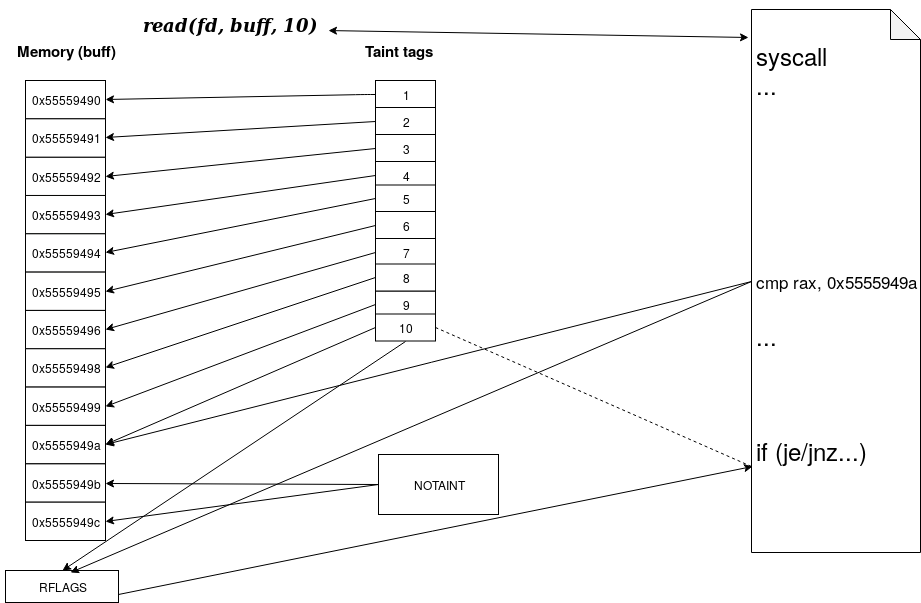
\includegraphics[scale=0.5]{img/source_tainting.png}
    }
    \caption{Создание пометок в \texttt{moflow gentrace}}
    \label{fig:moflow1}
\end{figure}

Теперь рассмотрим другой случай. Пусть после вызова \texttt{read(fd, buf, 10)} последует инструкция \texttt{mov rcx, qword ptr [rsi]}, где \texttt{rsi} хранит адрес \texttt{buf}. В то время как в действительности произошло побайтовое копирование, \texttt{moflow} видит это иначе.

\begin{itemize}
    \item Для каждого адреса или регистра, который читается в рамках инструкции берется соответствующая ему метка. Все полученные метки объединяются при помощи функции \texttt{combineTaint}.
    \item В каждый адрес или регистр, в которых во время инструкции происходит запись пишется метка, полученная в предыдущем пункте.
\end{itemize}

\begin{lstlisting}[environoment=cpp_code,captionpos=b]
uint32_t TaintTracker::combineTaint(uint32_t oldtag, uint32_t newtag)
{
  if (newtag) {// its tainted
    if (oldtag == NOTAINT)
      return newtag; // FIXME
    else 
      return MIXED_TAINT;
  }
  return oldtag;
}
\end{lstlisting}

Где \texttt{NOTAINT} это $0$ -- значение обозначающее, что метка отсутствует, а \texttt{MIXED\_TAINT} это $2^{32}-1$, обозначающее наличие более чем одной пометки.

\begin{figure}[H]
    \center{
        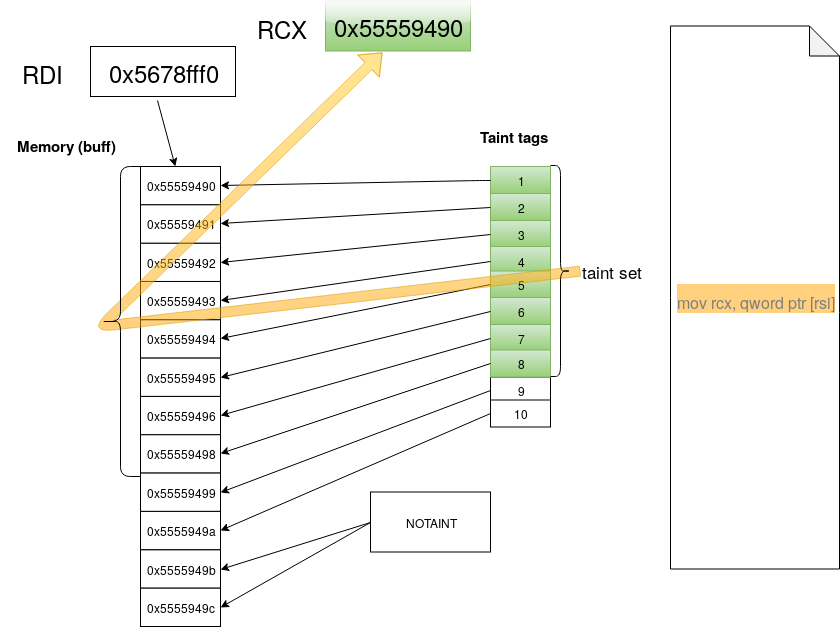
\includegraphics[scale=0.5]{img/propagation1.png}
    }
    \caption{Распространение пометок в \texttt{moflow gentrace}}
    \label{fig:moflow2}
\end{figure}

Таким образом, первое что необходимо реализовать это структуру \texttt{Множество меток}, которая должна поддерживать $3$ операции.

\begin{itemize}
    \item Добавление метки в \texttt{множество меток}.
    \item Объединение с другим \texttt{множество меток}
    \item Вывод содержимого Множества \texttt{множества меток}
\end{itemize}

Предположим теперь, что эта структура уже есть (далее будут описана её реализация). Допустим, встретилась еще одна инструкция копирования \texttt{mov word ptr [rdi], rcx}. \textbf{0x5678fff0} и \textbf{0x5678fff1}помечаются $8$ тегами. Правильно было бы представить \textbf{RCX} как 8 отдельных байт, которые могут быть помечены независимо, тогда \textbf{0x5678fff0} и \textbf{0x5678fff1} будут помечены $2$ различными тегами.

\begin{figure}[H]
    \center{
        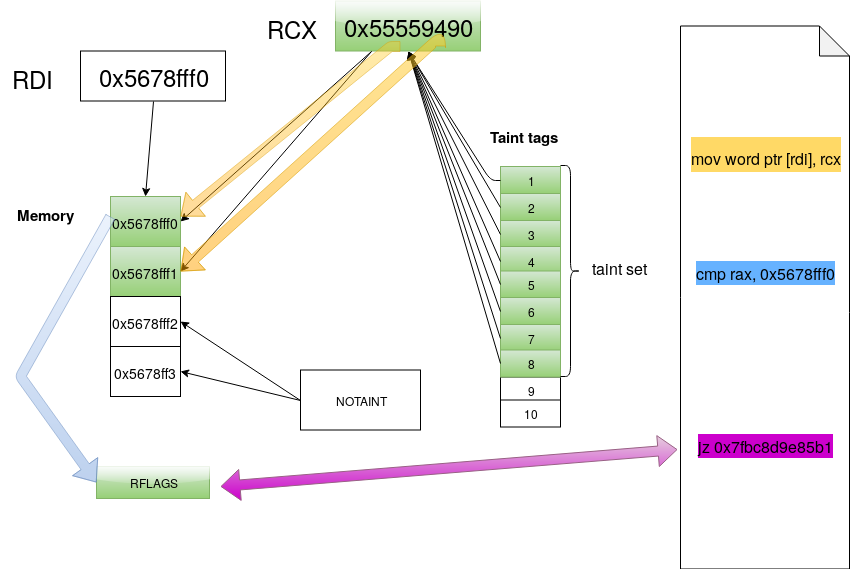
\includegraphics[scale=0.5]{img/propagation2.png}
    }
    \caption{Перепомечивание в \texttt{moflow gentrace}}
    \label{fig:moflow3}
\end{figure}

\section{Реализация \texttt{Множества Пометок}}

Наиболее простым и естественным решением, было бы использовать структуру данных реализующую интерфейс обычного множества в математическом смысле, в случае \texttt{C++} такой структурой данных является \texttt{std::set}. Тем не менее, непосредственные попытки использования вызвали ощутимые проблемы в производительности. Профилирование показало, что проблема в многочисленных аллокациях памяти, связанных c

\begin{itemize}
    \item Операцией объединения множеств
    \item Многочисленными аллокациями, вызванными необходимостью создавать временные множества пометок на каждую операцию распространения пометок
\end{itemize}

Дальнейший анализ показал, что на всех изученных примерах более чем в 70\% случаев соответствующие адресам и регистрам \texttt{множества пометок} оказываются пустыми или состоящими из одного элемента. Отсюда вытекает очевидная оптимизация. Будем представлять множество пометок в виде типа-суммы из двух элементов: \texttt{uint32\_t} и \texttt{tag\_set*}, где первый элемент используется как в оригинальном \texttt{gentrace}, то есть говорит об отсутствии метки, наличии единственной метки (в этом случае содержит её значение) или показывает, что меток более чем одна. В последнем случае используется непосредственно \texttt{tag\_set*}, в иных случаях значением второго элемента является нулевой указатель.

Не смотря на приведенную выше оптимизацию, остаётся необходимость реализовать структуру реализующую само множество. Были рассмотрены следующие варианты его реализации:


\subsection{Динамический массив}

В данной реализации был использован \texttt{std::vector} из стандартной библиотеки \texttt{C++}. При этом 
\begin{itemize}
    \item Добавлению соответствует операция добавления элемента в конец вектора.
    \item Объединению запись второго вектора в конец первого, с последующим удалением дублирующих элементов\footnote{Были проведены эксперименты, для определения границы при превышение которой стоит начать удаление дублей. Результаты показали, что разница между порогом в 20 элементов и меньшими статистически не различима, в то время как большие значение показывают худший результат}
    \item Вывод значений производится итерацией по элементам вектора.
\end{itemize}

\subsection{Битовое множество фиксированного размера}

Использование битового множества, представляется достаточно логичным решением, поскольку это структура данных, позволяющая быстро выполнить объединение множеств за линейное время -- операция сводится к выполнению побитового или, для этой операции также можно использовать \text{SSE} инструкции, что также положительно сказывается на производительности. Другим его преимуществом является компактность для хранения достаточно больших множеств, так $1$ байт может хранить информацию о $8$ метках.

Недостатком является объем занимаемой памяти, кроме того объединение множеств из $2$ элементов занимает столь же много времени, как и объединение множеств максимального поддерживаемого размера. Таким образом, эта структура данных может быть достаточно эффективна, если приходится оперировать достаточно большими множествами или если количество используемых меток невелико. Однако в ситуации когда меток много, причем конкретные адреса помечены их небольшим количеством -- битовое множество оказывается уже не столь эффективной структурой.

В стандартной библиотеке присутствует только реализация битового множества фиксированного размера \texttt{std::bitset}. Поскольку количество элементов должно быть известно на этапе компиляции, этот подход в чистом виде не применим. Тем не менее он представляет интерес как некоторый ориентир, в тестах было использовано значение в $6000$, как наименьшее круглое значение которого достаточно для тестовых примеров.
При данном подходе для всех операций использовался естественный интерфейс битового множества.

В библиотеке \texttt{Boost} есть реализация такой структуры данных как \texttt{dynamic\_bitset}, которая позволяет устанавливать размер множества динамически, а также менять его. Тем не менее, это решает только проблему с необходимостью знать количество меток на этапе компиляции. Все остальные проблемы остаются актуальными.

\subsection{Использование сжатых битовых векторов}

Использование сжатие для битовых векторов, потенциально позволяет решить проблему с достаточно разряженными битовыми векторами, и эффективно хранить множества с малым количеством меток.
В такой структуры данных было принято решение использовать библиотеку \texttt{CRoaring} -- реализацию протокола сжатых битовых векторов \texttt{Roaring} \cite{Roaring}. Данная библиотека в целом аналогична обычному битовому множеству с точки зрения интерфейса, однако поддерживает операции над множествами разного размера. Реализация также использовала естественный интерфейс множества, предлагаемый библиотекой.


\subsection{Ассоциативный массив битовых множеств}

Основным недостатком битового множества является необходимость хранить множество пустых битов на отсутствующие элементы, а преимуществом - возможность очень быстрой операции объединения. Один из подходов, позволяющих избавиться от этого недостатка был рассмотрен в предыдущем пункте, другой основан на следующей идее.

Будем использовать ассоциативный массив (\texttt{std::map} из стандартной библиотеки), ключами которого являются целые числа, а значениями битовые вектора размера $N$. Пусть \texttt{T} описанный ассоциативный массив, рассмотрим реализацию операций, которые он должен поддерживать.


\begin{itemize}
    \item \texttt{Добавление элемента}. Пусть в \texttt{T} следует добавить элемент $x$. Возможны 2 случая
    \begin{itemize}
        \item \texttt{T} не содержит элемента с ключом $\floor*{\frac{x}{N}}$. Тогда в \texttt{T} добавляется элемент с соответствующим ключом и битовым вектором из нулей в качестве значения, затем элемент с номером $x \bmod N$ этом битовом векторе устанавливается в $1$.
        \item \texttt{T} содержит элемент с ключом $\floor*{\frac{x}{N}}$. Тогда у битового вектора, соответствующего этому ключу элемент c номером $x \bmod N$ устанавливается в $1$.
    \end{itemize}
    \item \texttt{Объединение множеств}. Пусть \texttt{T} следует объединить с $\texttt{T}_2$. Для элементов присутствующих и в $\texttt{T}_2$ и в \texttt{T} выполняется операция побитового или. Элементы, которые есть только в $\texttt{T}_2$ копируются в \texttt{T}.
    \item \texttt{Печать содержимого} производится естественным образом, совершается обход всего содержимого $T$, при этом если элемент $i$ в битовом векторе, соответствующем ключу $k$ установлен в $1$, то следует напечатать номер метки $k \cdot N + i$.
\end{itemize}

\subsection{Множество интервалов}

Существует еще один подход к реализации \texttt{множества меток}. Если некоторое множество состоит из последовательных чисел, то для его представления можно хранить только первый и последний элемент. Соответственно произвольное подмножества натуральных чисел можно представить как дизъюнктное объединение таких интервалов, где отдельно стоящие элементы представляются в виде пары из одинаковых чисел.

Использование подобной структуры имеет смысл в случае если обрабатываемые множества состоят из малого количества интервалов, что является достаточно разумным предположениям для помеченных данных.

В качестве реализации использовался модуль \texttt{boost::icl::interval\_set} из проекта \texttt{Boost}.


\subsection{Тестирование производительности различных реализаций}

Для тестирования производительности были использованы 4 различных приложения

\begin{itemize}
    \item \texttt{cmark} -- инструмент для преобразования markdown в html, написанная на \texttt{C}, входной файл из $3379$ байт, количество инструкций в трассе \numprint{608398}, количество операций над множествами меток \numprint{205273}.
    \item \texttt{file} -- инструмент из binutils, определяющий тип файла, входной файл содержит строку \texttt{``1123235235346436\textbackslash n''}, количество инструкций в трассе \numprint{14343775}, количество операций над множествами меток \numprint{23494644}.
    \item \texttt{jpeg} -- программа из набора \texttt{LAVA} \cite{LAVA} для обработки jpeg файлов, входной файл из $5770$ байт, количество инструкций в трассе \numprint{9043561}, количество операций над множествами меток \numprint{55839222}.
    \item \texttt{libyaml} -- программа из набора \texttt{LAVA} для обработки yaml файлов, входной файл из $5242$ байт, количество инструкций в трассе \numprint{11580028}, количество операций над множествами меток \numprint{11157748}
\end{itemize}

% \textbf{}\\
% \scalebox{0.8}{
\begin{table}[H]
    \caption{Время работы в секундах для различных реализаций} \label{tab:compare}
    \scalebox{0.8}{
    \begin{tabular}[]{@{}lllllllll@{}}
    \toprule
    & vanilla & vector & bitset6000 & roaring & bitset64 tree & bitset256
    tree & bitset512 tree & interval set \tabularnewline
    \midrule
    % \endhead
    cmark & 3.5s & 4.6s & 3.7s & 4.2s & 3.8s & 3.7s & 3.7s & 3.7s \tabularnewline
    file & 20.8s & 47s & 60s & 70s & 45.5s & 46s & 47s & 46s \tabularnewline
    libjpeg & 14.5s & 1762s & 49s & 378s & 307s & 108s & 80s & 165s \tabularnewline
    libyaml & 16.5s & 22.5s & 25s & 26s & 23.5s & 23.5s & 23.5s & 24s \tabularnewline
    \bottomrule
\end{tabular}}
\end{table}

Исходя из результатов в таблице \ref{tab:compare}, было принято решение остановиться на реализации с Ассоциативным массивом с $256$ битным битовым вектором. Код реализующий описанную структуру можно найти в приложении \ref{tagsetimpl}.

\section{Другие доработки}

Помимо реализации множества пометок было проделано еще несколько усовершенствований \texttt{Moflow gentrace}.

\subsection{Удаление не нужного функционала}

Целью изначального инструмента было сохранение трасс выполнения в формате \texttt{protobuf}, однако с точки зрения решаемой задачи в этом нет никакого необходимости. Более того, профилирование показало, что сохранение трассы ощутимо влияет на производительность.


\begin{table}[H]
    \centering
    \caption{Время работы с сериализацией и без} \label{tab:compare2}
    % \scalebox{0.4}{
    \begin{tabular}[]{@{}lll@{}}
    \toprule
    & с сериализацией трассы & без сериализации трассы  \tabularnewline
    \midrule
    % \endhead
    cmark & 3.7s & 3.4s \tabularnewline
    file & 46s & 29s \tabularnewline
    libjpeg & 108s & 99s \tabularnewline
    libyaml & 23.5s & 22s \tabularnewline
    \bottomrule
\end{tabular}
\end{table}

Как видно из таблицы \ref{tab:compare2} производительность инструмента существенно возросла. Из других преимуществ следует отметить упрощение кодовой базы, и возможность использовать версию \texttt{Pin 3.7} по причине отсутствия внешних зависимостей.

\subsection{Улучшения работы с помеченными данными}

В оригинальном инструменте не была реализована поддержка некоторых системных вызовов под операционной системой Linux. Была добавлена поддержка \testtt{pread64}, \texttt{socket} и \texttt{recvfrom}.

Также была реализована возможность указания произвольной гранулярности меток и возможность использовать разметку входного файла для помечивания. Остановимся на второй возможности чуть подробнее. 
В пункте \ref{taintmethod} упоминалась возможность использования \texttt{afl-analyze}, чтобы определить семантику использования некоторых байтов входного файла. Был разработан вспомогательный инструмент на языке \texttt{Python}, обрабатывающий вывод \texttt{afl-analyze} c целью генерирования файла разметки. В \texttt{}
% \input{report.tex}
% \vbox{
%     \centering
%     \includegraphics[width=476]{titil.pdf}
%     % \maketitle %this typesets the contents of \title, \author and \date
% }
\clearpage
% \begin{figure}
%  \centering 
%  \includegraphics{titil.pdf}
% % \end{figure}
% \input{titul.tex}
% % {\bfseriesАннотация}

% {\large В работе рассматривается возможность расширения функциональности
% механизма контроля поведения программ, используемого в SELinux, при
% помощи повышения гранулярности контроля поведения приложений
% в указанной системе за счет отслеживания внутреннего состояния
% программы из ядра. Предлагается делать это при помощи
% разметки исполнимого кода приложения контрольными точками
% на уровне исходных текстов.
% }

\newpage
\tableofcontents
\newpage

\bigskip
\section{Введение.}

В месте с распространением современных средств разработки программного обеспечения, растет также и сложность производимых программных продуктов. Поиск ошибки в программе большого размера может быть достаточно нетривиальной программой. Для облегчения этой задачи активно используется и разрабатываются отладчики. Одним из наиболее известных развиваемых и продвинутых является ~\cite{gdb}, разработанный в конце прошлого столетия Ричардом Столлменом для проекта GNU.

Символьное выполнение - набирающее популярность в последние годы техника, впервые использованная
в середине 70ых с целью верификации программного обеспечение. Сразу после появления это была достаточно теоретическая область, т.к. символьное выполнение в конечном итоге сводится
к задаче выполнимости булевых формул (SAT), которая как известно, является NP полной.
Рост производительности вычислительной техники в последние годы сделал возможным применение методов символьного выполнения на практике.

\section{Постановка задачи}
\subsection{Расшифровка темы}
Исследовать существующий инструментарий в области символьного выполнения, используемый для отладки программного обеспечение.
Разработать инструментарий, облегчающий отладку с использованием методов символьного выполнения.

\begin{itemize}

\item Изучить стандарт SMT-LIB\cite{smtlib} для работы с SMT решателями
\item Изучить методы транслирования промежуточных языков в формулы для SMT решателей в соответствии со стандартом SMTLIB2.
\item Провести анализ существующих средств символьного выполнения, применимых для задач отладки программ/анализа двоичного кода.
\item Провести анализ возможностей расширения gdb для интеграции со средствами символьного выполнения.
\item Провести анализ возможностей расширения radare2 для интеграции со средствами символьного выполнения.
\item Разработать библиотеку для трансляции бинарного кода в smt-lib2.0

\end{itemize}

\subsection{Актуальность}

Как уже было сказано в введении, сейчас область символьного выполнения активно развивается.
Однако несмотря на наличие инструментария для символьного выполнения бинарного кода, применение соответствующих средств для интерактивной отладки практически не используется.

\subsection{Цель работы}

Исследовать существующие методы символьного выполнения, применимые к задаче отладки программ, провести их анализ
Изучить существующий инструментарий, произвести его доработку или разработать на его основе решение для отладки.

\section{Обзор предметной области}

\subsection{Обзор символьного выполнения}

\subsubsection{общие концепции}

Хороший и достаточно полный обзор символьного выполнения, от истории до применений и основных подходов можно найти в \cite{SurveySymExec-CSUR18}.

Символьное выполнение представляет собой способ выполнения программы, при котором вместо конкретных значений переменных используются символьные. В то время как значением обычной переменной является некоторое значение соответствующего ей типа, символьное переменная представляет собой формулу, задающую некоторое множество значений.
Соответственно операция над символьной переменной - это операция над соответствующей ей формулой.
\bigskip
Подобно тому, как состояние обычной программы в процессе своего выполнения характеризуется множеством значений переменных и инструкции, которая подлежит выполнению следующей (в большинстве существующих процессоров адрес следующей инструкции явно хранится в соответствующем регистре, то есть текущее состояние процесса целиком характеризуется содержимым памяти).
Аналогичный подход используется и при символьном выполнении.
Обычно движок символьного выполнения оперирует над тройками $(stmt,~\sigma,~\pi)$, где

\begin{itemize}
\item $stmt$ это следующее выражение, которое будет исполнено. Это может быть как конкретный адрес, так и некоторая формула с условным переходом.

%\item $\sigma$ is a {\em symbolic store} that associates program variables with expressions over \mynote{[D] $\alpha_i$ also concrete?} concrete and symbolic values $\alpha_i$.

\item $\sigma$ это контейнер, моделирующий память процесса. Он содержит выражения описывающие возможные состояния символьных переменных.

\item $\pi$ это {\em ограничения пути}, некоторая формула над переменными из $\sigma$, значение которой истинно тогда и только тогда, когда $stmt$ - следующее выражение подлежащее выполнению.

\end{itemize}

Несмотря на то, что идея выглядит достаточно простой, на практике существует ряд сложностей.

\begin{itemize}
%%%
\item \noindent {\em Память}: Как работать с массивами и указателями?

\item {\em Взаимодействие с инфраструктурой}: Что делать с библиотечными функциями/системными вызовами?

\item {\em Побочные эффекты и внешнее окружение}: Что делать с побочными эффектами? Изменением файлов и отправкой/получением сетевых пакетов?

\item {\em Экспоненциальный рост путей и состояний}: Размер и соответственно сложность формул зависят экспоненциально от размера программы.

\end{itemize}

Работа непосредственно с двоичным кодом также вносит дополнительные сложности, растет как размер формул по сравнению с логически эквивалентным высокоуровневым кодом, так и сложность работы с памятью, ввиду отсутствия соответствующих абстракций.

\bigskip

\subsubsection{SMT-решатели}

Выше приведено достаточно абстрактное описание символьного выполнения, на практике необходим инструмент способный эффективно работать с формулами. В качестве такого инструмента обычно используются SMT-решатели.
{\em SMT} расшифровывается как {\em satisfiability modulo theories}, то есть задача проверки выполнимости теорий первого порядка. Существует достаточно много SMT-решателей,
в частности можно отметить {\em Z3} \cite{Z3}, {\em CVC3} \cite{CVC3} и {\em Alt-Ergo} \cite{Alt-Ergo}.

\bigskip

Поскольку SMT-решатели являются достаточно зрелой технологией, существует стандарт \em {SMT-LIB2.0} \cite{smtlib}, описывающий специальный lisp-подобный DSL, поддерживаемый всеми серьезными инструментами. В настоящее время последней версией стандарта является версия $2.6$.

Сам стандарт достаточно богат возможностями, однако для целей данной курсовой достаточно теории
битовых векторов, поскольку это в точности соответствует формату в котором переменные хранятся в памяти.

{\bf Пример} (из документации Z3)
\begin{lstlisting}
(define-fun is-power-of-two ((x (_ BitVec 4))) Bool
(= #x0 (bvand x (bvsub x #x1))))
(declare-const a (_ BitVec 4))
(assert
(not (= (is-power-of-two a)
(or (= a #x0)
(= a #x1)
(= a #x2)
(= a #x4)
(= a #x8)))))
(check-sat)
\end{lstlisting}

В этом примере доказывается что $x \:\&\: (x - 1)$ верно тогда и только тогда, когда $x$ является степенью двойки (для битовых векторов длинной 4). Как можно видеть, язык SMT-LIB в случае битовых векторов достаточно прост:

\begin{itemize}
%%%
\item \noindent {\em define-fun}: Определение функции.

\item {\em define-const}: Частный случай {\em define-fun}, функция без аргументов, давно поддерживается {\em Z3}, но не так давно появился в стандарте. Вместо
\begin{verbatim}(declare-const a (_ BitVec 4))\end{verbatim}
можно использовать
\begin{verbatim}(define-fun a () (_ BitVec 4))\end{verbatim}

\item {\em assert }: Проверка истинности формулы

\item {\em check-sat }: Проверка разрешимости существующих формул

\item {\em get-model }: Получить значения переменных, при которых теория разрешима.

\end{itemize}

Остальные функции представляют собой операции над битовыми векторами.

\bigskip

Помимо непосредственного использования SMT-LIB, можно использовать различные библиотеки для работы с SMT-решателем из языка программирования.

Множество примеров непосредственной работы с SMT-решателями можно найти в \cite{yusmt}.


\subsection{Обзор инструментов для отладки}

Поскольку в данной курсовой, символьное выполнение рассматривается в приложении к конкретной задаче - необходимо также рассмотреть существующие отладчики.

\subsubsection{gdb}

Gdb \cite{gdb} - расшифровывается как GNU Debugger, это стандартный отладчик проекта GNU.
Gdb является отладчиком уровня исходного кода, он подразумевает что программа была скомпилирована с отладочными символами и целиком поддерживает интеграцию с ними, позволяя делать шаги не по ассемблерным инструкциям, а по шагам исходного кода, ставить брекпоинты по имени функции, показывать номер строки и т.д.

Стандартный режим работы gdb использует системный вызов {\em ptrace}, который позволяет отслеживать состояние процесса.

\begin{figure}[h]
\centering
\includegraphics[width=80mm, scale=0.5]{gdb-structure.png}
\caption{Устройство Gdb}
\label{fig:gdb1}
\end{figure}

Важным достоинством gdb является его поддержка плагинов, возможно разработка расширений на языке python, значительно облегчающих отладку. Что делает gdb отличным выбором для расширения посредством добавления возможностей символьного выполнения.

Ниже пример популярного gdb плагина

\begin{figure}[h]
\centering
\includegraphics[width=120mm, scale=1]{gdb-dashboard.png}
\caption{GDB dashbord плагин}
\label{fig:gdb2}
\end{figure}

\subsubsection{radare2}

Radare2 \cite{r2} - свободный фреймворк для обратной разработки. Следуя философии UNIX он состоит из набора независимых утилит командной строки

\begin{itemize}
%%%
\item \noindent {\em radare2 (r2)}: Ядро шестнадцатеричного редактора и отладчика, позволяет открывать файлы, диски, сетевые соединения, модули ядра, процессы для отладки и т.д. Также содержит продвинутый интерфейс для манипуляций с открытым объектом. В том числе визуализацию, анализ, патчи двоичного кода, дизассемблирование и т.д. Кроме того может быть расширен посредством плагинов на различных языках программирования, в частности на {\em python}.

\item {\em rabin2}: Утилита для извлечения информации из различных форматов исполняемых файлов.
В случае ELF является аналогом readelf,

\item {\em rasm2 }: Ассемблер и дизассемблер для множества архитектур, позволяет как получить двоичное представление для команд ассемблера или байт-кода виртуальной машины, так и произвести обратное преобразование.

\item {\em rahash2}: Универсальная утилита для хэширования, позволяет вычислять различные виды хэш функций для строк, файлов и т.д. Обычно используется для проверки целостности.

\item {\em radiff2 }: Поддерживает различные алгоритмы для сравнения двоичных файлов.

\item {\em rafind2 }: Программа для поиска определенных последовательностей байт в файле.

\item {\em ragg2 }: Компилирует программы на специальном мини языке высокого уровня в исполняемые двоичные файлы для архитектур x86, amd64 и ARM.

\item {\em rarun2 }: Программа для запуска процессов в различных окружениях, с различными переменными окружения, правами и т.д. Используется для фаззинга и тестирования.

\item {\em rax2 }: Минималистичная утилита для конвертирования чисел из разных представлений друг в друга.

\end{itemize}

Ниже пример визуального интерфейса radare2

\begin{figure}[h]
\centering
\includegraphics[width=150mm, scale=2]{r2-example.png}
\caption{визуальный режим radare2}
\label{fig:r2a}
\end{figure}

\bigskip

Radare2 позволяет для любой команды получить её вывод в json, а также подеррживает режим работы через именованный канал. Вместе эти два свойства делают возможными как встраивание radare2 в другие программы, так и создание альтернативных интерфейсов для него (в настоящее время активно развивается веб-интерфейс, и декстопный интерфейс на Qt).
Кроме того radare2, как и gdb поддерживает плагины, позволяющие расширить его возможности новыми командами.

Однако, наиболее интересным для данной работы свойством radare2 является язык промежуточного представления ({\em IR}) {\em ESIL}.

Esil расшифровывается как Evaluable Strings Intermediate Language и отчасти похож Forth. Он не предназначен для удобства чтения человеком, а предполагает выполнение на специальной виртуальной машине Esil (EVM).
Это приводит к определенным сложностям, о которых будет рассказано в соответствующем разделе.

\subsubsection{Triton}

Наконец важно отметить инструмент {\em Triron} \cite{Triton}. Он представляет собой фреймворк для динамического анализа двоичных приложений посредством символьного выполнения. Можно сказать, что в нем реализованы как раз те теоретические подходы, что обсуждалиcь выше.

Cимвольный движок Triton управляет

\begin{itemize}
%%%
\item Таблицей с состояниями символьных регистров

\item Хэш таблицей с символьным состоянием памяти.

\item Глобальным множеством символьных ссылок.

\end{itemize}

Во время выполнения, таблица с символьными регистрами обновляется после каждого шага в соответствии с соответствующей семантикой, аналогичное происходит и для остальной памяти. Кроме того, важно отметить, что triton также оперирует и конкретными значениями, когда это возможно.



\begin{figure}[h]
\centering
\includegraphics[width=120mm, scale=1]{triton_architecture.jpg}
\caption{Устройство Triton}
\label{fig:triton1}
\end{figure}

%(e.g., the maximum size of a buffer or the number of iterations for a loop).
%%%

\section{Обзор существующих решений}

\bigskip

Так как в ходе работы планировалось использовать Intermediate Language, чтобы
избежать привязки к какой-либо архитектуре, вначале был рассмотрен инструментарий относящийся к radare2 - фреймворку для обратной разработки.

\subsection{Rune}
\{\em Rune} \cite{Rune} - инструмент созданный нный для целей схожих с целями данной работы. Был сделан преимущественно летом 2017 в рамках Google Summer of Code (GSOC). Представляет собой движок символьного выполнения, работающий поверх ESIL.
% https://github.com/radare/rune/tree/master

Написан на языке Rust.
В качестве зависимостей имеет только несколько вспомогательных Rust библиотек и непосредственно radare2, c которым идет взаимодействие через pipe.

Формально находиться в разработке, однако последние значимые доработки были в рамках GSOC2017, на данный же момент явно заброшен

Слабо документирован, падает с паникой в большинстве случаев вместо сообщения об ошибке.

В ходе исследования Не удалось заставить его работать. Ниже пример интерактивной сессии работы в программе.

\begin{figure}[h]
\centering
\includegraphics[width=150mm, scale=1]{rune.jpg}
\caption{Пример работы с Rune}
\label{fig:rune}
\end{figure}

\subsection{Pimp}

Другим решением, также основанным на radare2 является pimp \cite{pimp}. Это плагин, написанный на python и использующий triton для взаимодействия с smt решателем. К сожалению, инструмент заброшен и находится в стадии proof of concept (всего 600 строчек). Единственные его упоминания относятся к докладу на конференции ради которого он и был разработан.

Документация также отсутствует. Интерфейс не является интуитивным.

% https://github.com/kamou/pimp

% Написан на python, взаимодействует и с r2

\subsection{symgdb}

Несколько иным решением является symgdb \cite{symgdb}. Это плагин к gdb \cite{gdb}, никак не связанный с radare2. Из всех трех он является наиболее проработанным, в частности он должен позволять использовать конкретные значения переменных из текущего стекового кадра в gdb без дополнительных усилий.

Плагин написан на python и использует triton для трансляции в бинарного кода
в smtlib формат и взаимодействия с SMT решателем.

К сожалению, он также заброшен, а кроме того работает только с устаревшей версией triton и требует особой версии gdb, собранной с поддержкой python2.

Таким образом, ни один из существующих инструментов не решает поставленную задачу. Тем не менее сам факт их создания говорит о её актуальности.

\section{Проделанная работа}

\subsection{Выбор программного стека}

Для реализации практического инструментария для отладки, на начальном этапе было принято решение использовать IR, так как это 


\begin{itemize}
%%%
\item Позволяет получить непривязанный к конкретной архитектуре инструмент.

\item IR являются более простыми и удобными для анализа чем машинный код.

\end{itemize}

В качестве такого IR языка был выбран ESIL, по причине растущей популярности radare2, а также активному развитию непосредственно ESIL.

В качестве языка для рзработки был выбран python, как язык позволяющий быстро прототипировать решение и поддерживающий интеграцию с упомянутыми ранее технологии, то есть имеющий библиотеки для работы с различными решателями, а также radare2 и gdb.

Решение использовать triton было отложено на начальном этапе из образовательных целей, поскольку в нем уже реализована трансляция бинарного кода в smt формулы, представляющая отдельный интерес.


\subsection{Ход работ}

В начале была предринята попытка непосредственно провести синтаксический анализ ESIL кода, а потом полученное абстрактное синтаксическое дерево механически транслировать в SMT-LIB формат.

В ходе реализации, была обнаружена упомянутая выше проблема - ESIL предназначен для выполнения на EVM, и информация о значениях флагов в x86 в нем отсутствует, так как она неявно реализована в самой виртуальной машине.

\bigskip
Изучение исходных кодов Rune показало, что там для генерации SMT формул используется дополнительное промежуточное представление, реализованное в библиотеке esil-rs \cite{esil-rs}.
В нем команды изменяющие регистр флагов присутствуют явно.
Для использования этого промежуточного языка был написан python модуль \cite{pyesil}, позволяющий получить внутреннее представление из esil-rs в качестве последовательности s-выражений.


\bigskip

В качестве библиотеки для работы с SMT решателем была выбрана pysmt \cite{pysmt}, как не привязанная ни к одному конкретному решателю.

Наконец, был написан механизм транслирования SMT формул c использованием SSA на каждое присваивание.


\subsection{Архитектура полученного решения}

Текущая реализация с некоторым упрощением представляет собой следующий набор классов. 

\begin{itemize}
%%%
\item {\em InstructionSequence }: Класс, содержащий в себе состояние символьных переменных, а также ограничений на них. Содержит методы для объявления и модификации символьных переменных, а также непосредственно запуска SMT решателя. Инкапсулирует в себе целиком взаимодействие с решателем через pysmt.

\item {\em Token}: Вспомогательный класс, использованный при лексическом и синтаксическом анализе внутреннего представления Esil-rs.

\item {\em Ast }: Класс представляющий собой дерево дерево разбора esil-rs, используется при трансляции.

\item {\em Translator}: Класс, позволяющий обходить AST, генерируя формулы посредством InstructionSequence.

\item {\em SymbolicExecutor}: Класс, отвечающий за взаимодействие с radare2 и транслятором. Позволяет пошагово выполнять символьные инструкции, ставить хуки произвольного вида и обновлять/сбрасывать состояние InstrictionSequnce.

\end{itemize}

На основе вышеописанного уже можно писать плагин для gdb/radare2, что может быть проделано в дальнейшем.

\subsection{Проблемы}

В ходе реализации был выявлен ряд проблем, как фундаментального характера так и обусловенный выбранным стеком технологий. 

\begin{itemize}
%%%
\item {\em Отсутствие поддержки системных вызовов/сторонних библиотек}. Esil и основанный на нем esil-rd никак не обрабатывают такие ситуации. Однако, использование информации об оригинальных инструкциях и хуков позволяет реализовать эту поддержку пользователю самостоятельно.

\item {\em Множество esil команд соответствует одной команде процессора}. Поскольку выбор текущей команды основан на значении указателя инструкции нет возможности возникают сложности с ветвлениями, где одному адресу соответсвтует множество еsil команд, содержащее ветвление в рамках esil.

\end{itemize}


% https://github.com/SQLab/symgdb

\chapter*{Заключение}
\addcontentsline{toc}{chapter}{Заключение}

В данной работе было проведено исследование методов динамического анализа и выявлены два различных подхода для определения входных данных влияющих на выполнение условных переходов.

\begin{itemize}
    \item Подход на основе динамического символьного выполнения.
    \item Подход на основе динамического анализа помеченных данных.
\end{itemize}

Проведен анализ существующих инструментов динамического анализа с точки зрения применимости к поставленной задаче. Было принято решение использовать инструменты \texttt{Angr} и \texttt{Moflow gentrace} для реализации методов на основе динамического символьного выполнения и динамического анализа помеченных данных соответсвенно.

Была написана и протестирована на искусственных примера программа, использующая инструмент \texttt{Angr}. К недостатком полученной реализации следует отнести низкую производительность \texttt{Angr} в контексте решаемой задачи, а также невозможность мастшабировать решение на программы большего размера.
Метод на основе динамического анализа помеченных данных был программно реализован посредством доработок инструмента \texttt{Moflow gentrace}, данное решение обладает достаточной производительностью и может использоваться для анализа используемых в индустрии приложений. Тестирование проводилось на на наборе \texttt{LAVA} и программах с открытым исходным кодом (cmark).

% Таким образом поставленная задача в рамках работы решена.

В качестве дальнейших направлений развития работы можно назвать следующие:

\begin{itemize}
    \item Исследование возможностей оптимального использование фаззером полученной информации.
    \item Доработка модулей \texttt{Angr} с целью использования конкретного выполнения, исследование возможностей масштабирование средств динамического символьного выполнения на программы большего размера.
    \item Исследование возможностей улучшения точности инструмента анализа помеченных данных.
\end{itemize}


% В процессе решения поставленной задачи 
% \begin{itemize}

% \item Был проведен краткий обзор истории и современного состояния стандарт SMT-LIB\cite{smtlib} для работы с SMT солверами.
% \item Были исследованы методы транслирования промежуточных языков в формулы  формулы для SMT солверов в соответствии со стандартом SMTLIB2.
% \item Был проведен анализ существующих средств символьного выполнения, применимых для задач отладки программ/анализа двоичного кода.
% \item Был проведен анализ возможностей расширения gdb для интеграции со средствами символьного выполнения.
% \item Был проведен анализ возможностей расширения radare2 для интеграции со средствами символьного выполнения.
% \item Была разработана библиотека на языке python для трансляции бинарного кода в формат smt-lib2.0.


% \end{itemize}

% Была разработана python библиотека,
% позволяющая в простейших случаях осуществлять трансляцию бинарного кода кода в smt формулы, с использованием radare2 и вспомогательных библиотек для него.


\bigskip

% \bibliographystyle{abstract}
\bibliographystyle{ieeetr}
\bibliography{master-thesis}

\ma
\appendix
\chapter{Программный код решения на основе \texttt{Angr}}
\label{angrimpl}
% the \\ insures the chapter title is centered below the phrase: AppendixA

\begin{lstlisting}[environoment=py_code, caption=taint\_influence.py, captionpos=b]
#!/usr/bin/env python3

import sys
import argparse
from pprint import pprint
from collections import (
    OrderedDict,
    defaultdict,
    namedtuple,
)
from itertools import (
    takewhile,
    chain,
)
from functools import reduce

from helpers import (
    show_info,
    BinaryInfo,
    show_rip,
)

import claripy
import angr
import r2pipe

from networkx.algorithms import (
    all_shortest_paths,
)


SIZE = 20

Interval = namedtuple('Interval', ['start', 'end', 'size'])
BufferInfo = namedtuple('BufferInfo', ['data', 'size'])


def tainted_dict(constraints):

    def merge(args):
        new = defaultdict(set)
        for k in set(chain(*(a.keys() for a in args))):
            for arg in args:
                if k in arg:
                   new[k] |= arg[k]

        return new

    if isinstance(constraints, list):
        return merge(
            [tainted_dict(c) for c in constraints]
        )

    bv_info = namedtuple('bv_info', ['name', 'size'])

    def bits2bytes(bitset_buffer: BufferInfo):
        return reduce(
            lambda acc, bit: (
                acc | { bitset_buffer.size // 8 - (bit // 8) - 1 }
            ),
            bitset_buffer.data,
            set()
        )

    def parse_name(name):
        data = name.split('_')
        size = data[-1]
        original = data[:-2]
        return bv_info('_'.join(original), int(size))

    def operate(node):
        if node.op == 'Extract':
            start, end, parent = node.args
            start, end = sorted((start, end))
            parent_info = parse_name(parent.args[0])
            return parent_info.name, (start, end, parent_info.size)
        elif node.op == 'BVS':
            vector_info = parse_name(node.args[0])
            return vector_info.name, (0, vector_info.size - 1, vector_info.size)

    def get_leafs(ast, buff=None):

        def is_leaf(node):
            return node.op == 'BVS' and isinstance(node.args[0], str)

        if buff is None:
            buff = set()

        if isinstance(ast, claripy.ast.base.Base):

            if ast.depth == 2 and ast.op == 'Extract':
                buff.add(ast)
                return
            elif ast.depth == 1 and ast.op == 'BVS':
                buff.add(ast)
                return
            elif is_leaf(ast):
                return

            for a in ast.args:
                get_leafs(a, buff=buff)

        return buff

    tainted_intervals = defaultdict(set)
    for node in get_leafs(constraints):
        name, data = operate(node)
        tainted_intervals[name].add(
            Interval(*data)
        )

    return {
        k: bits2bytes(
            reduce(
                lambda acc, val: BufferInfo(
                    acc.data | set(range(val.start, val.end + 1)),
                    val.size
                ),
                tainted_intervals[k],
                BufferInfo(set(), 0)
            )
        ) for k in tainted_intervals
    }


class Explorer(object):

    def __init__(self, binary, **options):
        super(Explorer, self).__init__()
        self.binary = binary
        self.project = angr.Project(
            binary.path,
            **options
        )
        if self.project.loader.main_object.pic:
            print('Binary has position indepenent code!')
            self.offset = self.project.loader.main_object.mapped_base
            self.binary.update_on_offset(self.offset)
        else:
            self.offset = 0
        self.argv = None
        self.entry = None
        self.sm = None
        self.cfg = None
        self.trace = []

    def build_cfg(self):
        self.cfg = self.project.analyses.CFG()

    def init_entry(self, **options):
        self.entry = self.project.factory.full_init_state(
            args=self.argv,
            **options
        )
        self.sm = self.project.factory.simgr(self.entry)

    def add_symbolic_file(self, name, size):
        content = claripy.BVS(
            name,
            size * 8
        )
        sym_file = angr.storage.file.SimFile(name, content)
        self.entry.fs.insert(
            name,
            sym_file
        )

    def symbolize_argv(self, size):
        sym = claripy.BVS(
            'argv_0',
            size * 8
        )
        self.argv = [self.binary.path, sym]

    def enable_trace(self):

        def store(state):
            self.trace.append(state.copy())

        self.entry.inspect.b(
            'irsb',
            when=angr.BP_BEFORE,
            action=store
        )

    def add_breakpoint(self, btype, action):
        self.entry.inspect.b(
            btype,
            when=angr.BP_BEFORE,
            action=action
        )

    def search_for(self, addr):
        self.sm.explore(find=addr)
        # try:
        return self.sm.found[0]
        # except:
        #     import ipdb
        #     ipdb.set_trace()

    def get_constraints(self, state):
        return state.solver.constraints

    def tainted_bytes(self, state):
        return tainted_dict(state.solver.constraints)

    def tainted_trace(self, state):
        for action in reversed(
            [a for a in state.history.actions if a.type == 'constraint']
        ):
            print('------------------------------')
            print(f'Basic block addr: {hex(action.bbl_addr)}')
            print(f'Instruction addr: {hex(action.ins_addr)}')
            print(f'Formula: {action.constraint.ast}')
            print(f'Tainted bytes: {tainted_dict(action.constraint.ast)}\n\n')

    def view_file(self, state, name):
        sym_file = state.fs.get(name)
        if sym_file is None:
            raise KeyError(f'Symbolic file with name {name} not exists')
        data, actual_size, new_pos = sym_file.read(0, SIZE)
        # import ipdb
        # ipdb.set_trace()
        print(data)
        print(state.solver.eval(data, cast_to=bytes))

    def get_function_node(self, name):
        return self.cfg.get_node(self.binary.func_map[name][0])

    def shortest_path_list(self, source, sink):
        return list(
            all_shortest_paths(
                self.cfg.graph,
                self.get_function_node(source),
                self.get_function_node(sink)
            )
        )



def parse_args():
    parser = argparse.ArgumentParser(
        description='Get tainted bytes for branches'
    )

    parser.add_argument(
        'binary',
        type=str,
        help='binary to analyse'
    )
    parser.add_argument(
        'func',
        type=str,
        help='function or adress to search'
    )
    parser.add_argument(
        '-s',
        '--symbolic_argv',
        action='store_true',
        help='symbolize argv if set'
    )
    parser.add_argument(
        '-S',
        '--file-size',
        default=SIZE,
        help='Size of symbolic files'
    )
    parser.add_argument(
        '-f',
        '--files',
        default=[],
        nargs='+',
        help='list of files to symbolize',
    )
    parser.add_argument(
        'args',
        nargs='*',
        default=None,
        help='argv for program to analyse',
    )
    return parser.parse_args()


if __name__ == '__main__':
    options = parse_args()

    e = Explorer(
        BinaryInfo(options.binary),
        load_options={'auto_load_libs': True}
    )

    if options.symbolic_argv:
        e.symbolize_argv(SIZE)
    elif options.args:
        e.argv = [e.binary.path, *options.args]

    e.init_entry(
        # add_options={
        #     'SYMBOLIC_INITIAL_VALUES',
        # }
    )

    # e.add_breakpoint('irsb', show_rip)

    # e.build_cfg()

    # import networkx as nx
    # from networkx import graph
    # import matplotlib.pyplot as plt

    # nx.draw(e.cfg.graph)
    # plt.show()

    # sys.exit(0)
    # import ipdb
    # ipdb.set_trace()

    # pprint([(x.name, hex(x.addr)) for x in e.cfg.kb.functions])

    file_size = int(options.file_size)
    for file in options.files:
        print(f'[+] Add symbolic file of size {file_size}')
        e.add_symbolic_file(file, file_size)
    if options.func.startswith('0x'):
        addr = int(options.func, base=16) + e.offset
    else:
        addr = e.binary.func_map[options.func][0]

    print(f'Search for {hex(addr)}')
    state = e.search_for(
        addr
    )
    pprint(e.get_constraints(state))
    x = e.tainted_bytes(state)

    print('------------')
    pprint(x)
    print('=====Trace=========')
    e.tainted_trace(state)
    print('===files====')
    for f in options.files:
        e.view_file(state, f)

\end{lstlisting}


\chapter{Программный код реализации \texttt{Множества пометок}}
\label{tagsetimpl}

\begin{lstlisting}[environoment=сpp_code, caption=tags.h]
#ifndef PROJECT_TAGS_H
#define PROJECT_TAGS_H

#include <map>
#include <bitset>

#define MIXED_TAINT 0xFFFFFFFF
#define NOTAINT 0

#define CHUNK_SIZE 256


typedef std::bitset<CHUNK_SIZE> bitmap;
typedef std::map<uint32_t, bitmap> tag_storage;

class tag_set {
public:
    explicit tag_set() : storage_() {};
    explicit tag_set(uint32_t tag);
    ~tag_set() = default;
    tag_set& operator|=(const tag_set& ts);
    void insert(uint32_t tag);
    friend std::ostream& operator<<(std::ostream &strm, const tag_set& ts);

    
private:
    tag_storage storage_;
};


class taint_tag {

public:
    friend std::ostream& operator<<(std::ostream &strm, const taint_tag& tag);
    friend taint_tag operator|(taint_tag left_tag, const taint_tag& tag);
    taint_tag& operator|=(const taint_tag& tag);
    explicit taint_tag();
    explicit taint_tag(uint32_t);
    taint_tag(const taint_tag& tag);
    ~taint_tag();
    taint_tag(taint_tag && tag);
    taint_tag& operator=(taint_tag && other);
    taint_tag& operator=(const taint_tag & other);
    uint32_t get_value() const;
    size_t size() const;
    bool empty() const;

    static uint64_t op_count;

private:
    tag_set* data_;
    uint32_t value_;
};
\end{lstlisting}

\begin{lstlisting}[environoment=сpp_code, caption=tags.cpp]
#include <iostream>
#include <fstream>

#include "tags.h"


tag_set::tag_set(uint32_t tag) {
    std::div_t tag_info = std::div(tag, CHUNK_SIZE);
    this->storage_ = tag_storage();
    bitmap chunk_ptr = bitmap();
    chunk_ptr.set(tag_info.rem);
    this->storage_.emplace(std::make_pair(tag_info.quot, chunk_ptr));
}


void tag_set::insert(uint32_t tag) {
    std::div_t tag_info = std::div(tag, CHUNK_SIZE);
    bitmap chunk = bitmap();
    chunk.set(tag_info.rem);
    this->storage_[tag_info.quot] |= chunk;
}

tag_set& tag_set::operator|=(const tag_set& ts) {
    for (auto it = ts.storage_.begin(); it != ts.storage_.end(); ++it) {
        this->storage_[it->first] |= it->second;
    }
    return *this;
}

std::ostream & operator<<(std::ostream &strm, const tag_set& ts) {
    strm << "{";
    int k = 0;
    for (auto it = ts.storage_.begin(); it != ts.storage_.end(); ++it) {
        for (int j = 0; j < CHUNK_SIZE; ++j) {
            if (it->second.test(j)) {
                if (k) {
                    strm << ",";
                }
                strm << j + it->first * CHUNK_SIZE;
                k++;
            }
        }
    }
    strm << "}";
    return strm;
}


taint_tag::taint_tag() {
    this->value_ = NOTAINT;
    this->data_ = nullptr;
}


taint_tag::taint_tag(const taint_tag &tag) {
    if (tag.value_ == MIXED_TAINT) {
        this->value_ = MIXED_TAINT;
        this->data_ = new tag_set();
        *this->data_ |= *tag.data_;
    }
    else {
        this->value_ = tag.value_;
        this->data_ = nullptr;
    }
}

taint_tag::taint_tag(taint_tag && tag) {
    if (tag.value_ == MIXED_TAINT) {
        this->value_ = MIXED_TAINT;
        this->data_ = tag.data_;
        tag.data_ = nullptr;
        tag.value_ = NOTAINT;
    }
    else {
        this->value_ = tag.value_;
        this->data_ = nullptr;
        tag.data_ = nullptr;
        tag.value_ = NOTAINT;
    }
}

taint_tag& taint_tag::operator=(taint_tag &&other) {
    if (this != &other) {
        if (this->data_ != nullptr) {
            delete this->data_;
        }
        if (other.size() > 1) {
            this->value_ = MIXED_TAINT;
            this->data_ = other.data_;
            other.data_ = nullptr;
            other.value_ = NOTAINT;
        } else {
            this->value_ = other.value_;
            this->data_ = nullptr;
            other.value_ = NOTAINT;
            other.data_ = nullptr;
        }
    }
    return *this;
}

taint_tag& taint_tag::operator=(const taint_tag & other) {
    if (this != &other) {
        if (this->data_ != nullptr) {
            delete this->data_;
        }
        if (other.size() > 1) {
            this->value_ = MIXED_TAINT;
            this->data_ = new tag_set();
            *this->data_ |= *other.data_;
        } else {
            this->value_ = other.value_;
            this->data_ = nullptr;
        }
    }
    return *this;
}

taint_tag::~taint_tag() {
    if (this->data_ != nullptr) {
        delete this->data_;
        this->data_ = nullptr;
    }
}

taint_tag::taint_tag(uint32_t value) {
    this->value_ = value;
    this->data_ = nullptr;
}

std::ostream & operator<<(std::ostream &strm, const taint_tag &tag) {
    if (tag.empty()) {
        strm << "{}";
    } else if (tag.value_ == MIXED_TAINT) {
        strm << *tag.data_;
    } else {
        strm << "{" << tag.value_ << "}";
    }
    return strm;
}

size_t taint_tag::size() const {
    if (this->value_ == MIXED_TAINT) {
        return MIXED_TAINT;
    } else {
        return this->value_ == NOTAINT ? 0 : 1;
    }
}

bool taint_tag::empty() const {
    return (this->value_ == NOTAINT);
}


taint_tag operator|(taint_tag left_tag, const taint_tag& tag) {
    left_tag |= tag;
    return left_tag;
}

taint_tag& taint_tag::operator|=(const taint_tag &tag) {
    this->op_count++;
    if (tag.value_ == NOTAINT) {
        // nothing to do here
    } else if (tag.value_ == MIXED_TAINT) {
        if (this->value_ == MIXED_TAINT) {
            *this->data_ |= *tag.data_;
        } else {
            this->data_ = new tag_set();
            *this->data_ |= *tag.data_;
            if (this->value_ != NOTAINT) {
                this->data_->insert(this->value_);
            }
            this->value_ = MIXED_TAINT;
        }
    } else {
        if (this->value_ == MIXED_TAINT) {
            this->data_->insert(tag.value_);
        } else if ((this->value_ == NOTAINT) || (this->value_ == tag.value_)) {
            this->value_ = tag.value_;
        } else {
            this->data_ = new tag_set();
            this->data_->insert(this->value_);
            this->data_->insert(tag.value_);
            this->value_ = MIXED_TAINT;
        }
    }
    return *this;
}


uint64_t taint_tag::op_count = 0;
\end{lstlisting}

% \begin{appendices}
%   \chapter{Consectetur adipiscing elit}
%   \chapter{Mauris euismod}
% \end{appendices}


\end{document}
